\documentclass[9pt, aspectratio=169]{beamer}
\usepackage{FiraSans}
\usetheme{metropolis}
\usepackage[utf8]{inputenc}
\usepackage{amsmath}
\usepackage{amsfonts}
\usepackage{amssymb}
\usepackage{multicol}
\usepackage{tikz}
\usepackage[T1]{fontenc} 
\usepackage[skins]{tcolorbox}
\author{Nicola Roman\`o - nicola.romano@ed.ac.uk}
\title{Quantitative analysis of biomedical images - an introduction}
\setlength{\fboxsep}{0pt}
\setbeamertemplate{caption}{\raggedright\insertcaption\par}
\setbeamertemplate {footline}{\begin{scriptsize}\hfill\insertframenumber ~of \inserttotalframenumber\kern1em\vskip5pt\end{scriptsize}}

%\setbeamercovered{transparent} 
%\setbeamertemplate{navigation symbols}{} 

\titlegraphic{\centering 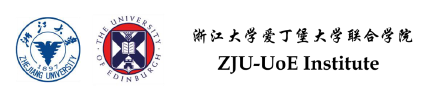
\includegraphics[scale=.5]{instituteLogo.png}}
%\institute{} 
\date{}
%\subject{} 

\begin{document}

\newtcolorbox{codebox}{enhanced,
	top=2pt,
	left=2pt,
	right=2pt,
	bottom=2pt,
	boxrule=0pt,
	leftrule=5pt,
	sharp corners,
	colback=gray!20,
	colframe=blue!60!black}

\begin{frame}
	\titlepage
\end{frame}

\begin{frame}
	{Learning objectives}
	At the end of this lecture you should be able to:
	\begin{itemize}
		\item Describe images as vectors and perform basic manipulation and visualization using Python
		\item Describe and explain how information is stored in images
		\item Explain and make use of basic concepts in image analysis such as SNR, histograms, LUT, \dots
	\end{itemize}
\end{frame}

\begin{frame}
	{What can (biomedical) image analysis tell us?}
	\begin{enumerate}
		\item Images are a big source of information
		\item Analysis can be \textbf{qualitative} or \textbf{quantitative}
	\end{enumerate}
	\pause
	\begin{columns}[T]
		\begin{column}{0.4\textwidth}
			\centering
			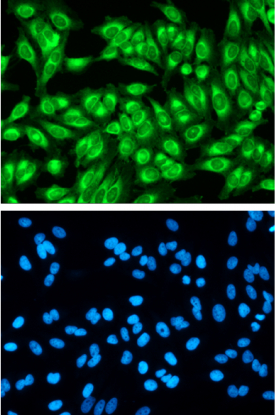
\includegraphics[height=150pt]{cells.jpg}
		\end{column}
		\pause
		\begin{column}{0.6\textwidth}
			\textbf{Qualitative:}
			\begin{itemize}
				\item Spindle-shaped cells
				\item Similar in size
			\end{itemize}
			\pause
			\textbf{Quantitative}
			\begin{itemize}
				\item Number of cells
				\item Position
				\item Size
				\item Staining intensity
				\item ...
			\end{itemize}
		\end{column}
	\end{columns}
\end{frame}

\begin{frame}
	{Images as matrices of pixels}
	In biomedical sciences, we deal with \textbf{raster images}, rectangular grids of pixels with varying intensity.

	\begin{figure}
		\centering
		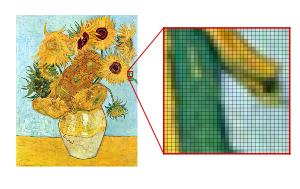
\includegraphics[height=150px]{vangoghzoom.png}
		\caption{Sunflower, Vincent Van Gogh (not a biomedical image, yet a pretty one!)}
	\end{figure}
\end{frame}

\begin{frame}
	{Representing matrices in Python}
	If working with matrices in Python, an obvious choice is using the NumPy library.

	NumPy is a Python open-source library for numerical computing, with support for n-dimensional arrays and many functionalities to work with matrices.
\end{frame}

\begin{frame}
	{Our first NumPy matrix!}

	\begin{codebox}
		\texttt{\# This is the standard way of importing numpy\\
			import numpy as np\\
			a = np.array([1, 2, 3])
		}
	\end{codebox}

	\begin{figure}
		\centering
		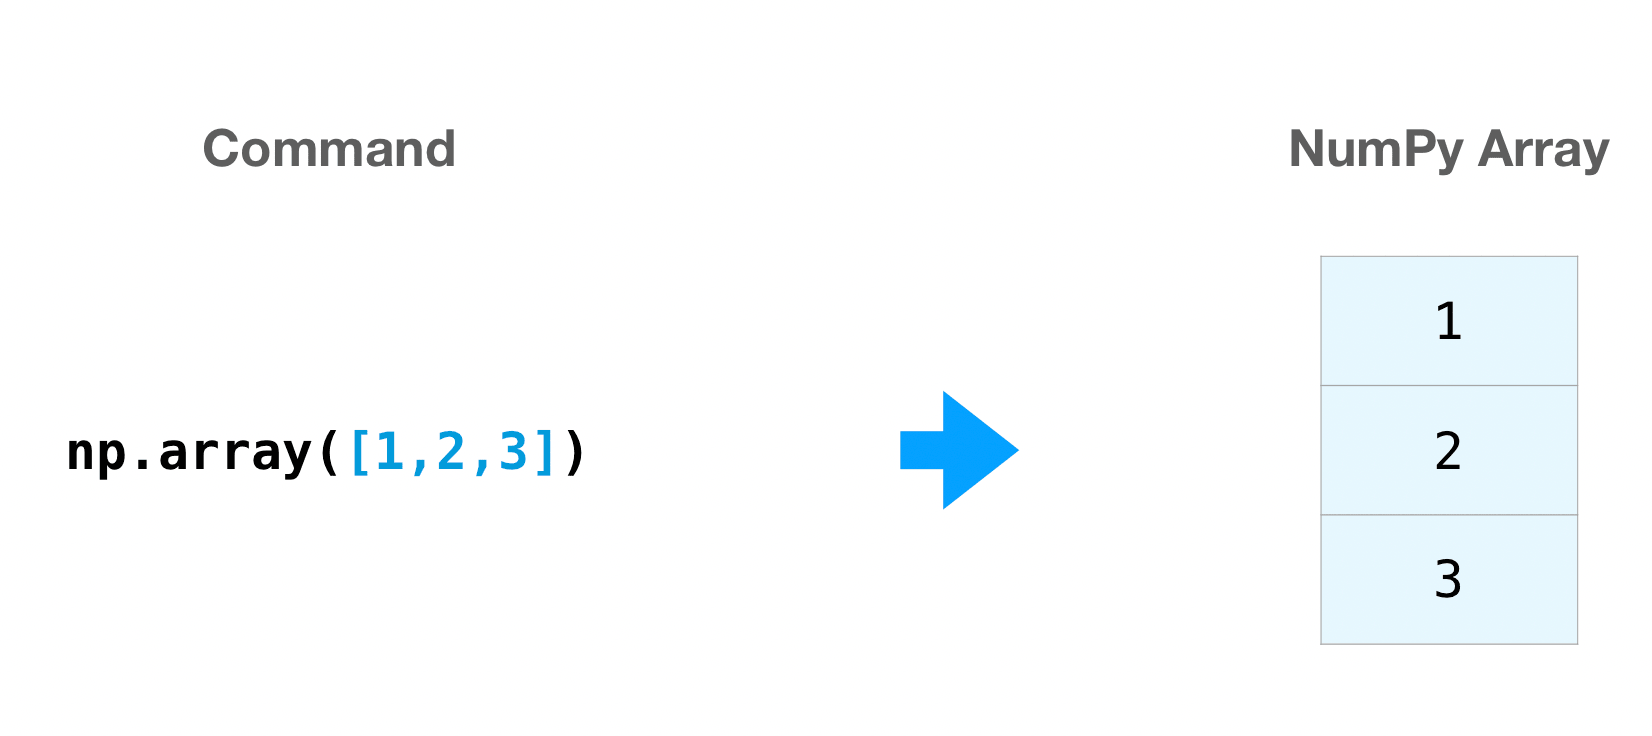
\includegraphics[height=100px]{np_array.png}
	\end{figure}
\end{frame}

\begin{frame}
	{Multiple dimensions}

	Numpy supports n-dimensional arrays with any number of dimensions.

	\begin{codebox}
		\texttt{import numpy as np\\
			b = np.array([[1, 2, 3][4, 5, 6]])\\
			print(b.shape)
		}
	\end{codebox}

	\begin{codebox}
		{
			\texttt{(2, 3)}
		}
	\end{codebox}

	The shape of an array is a vector showing the number of element in each of the dimensions of the array. In this case we have a matrix of 2 rows and 3 columns.
\end{frame}

\begin{frame}
	{Not just 2D!}
	Biomedical images are not limited to 2 dimensions!
	Three and >3-dimensional imaging is becoming more common.
	\pause
	Examples of other dimensions may include:
	\begin{itemize}
		\item z-axis
		\item time
		\item channels
		\item wells (for multiwell plate imaging)
	\end{itemize}
	\pause
	These can also be stored as n-dimensional matrices! Note that the axes order in the file may vary depending on the software used to create images.
	\begin{figure}
		\centering
		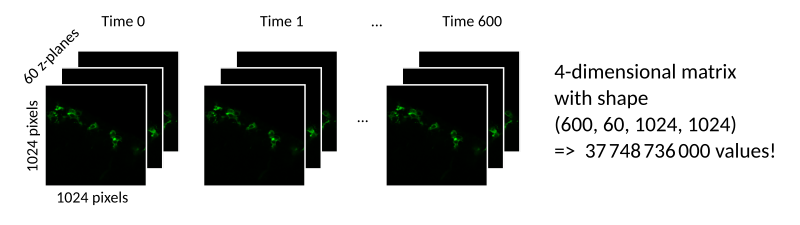
\includegraphics[width=\textwidth]{multidimensional.png}
	\end{figure}
\end{frame}

\begin{frame}
	{Array operations}

	Numpy allows matrix operations, selection of sub-matrices and much more, which can be used to manipulate our images.

	\begin{figure}
		\centering
		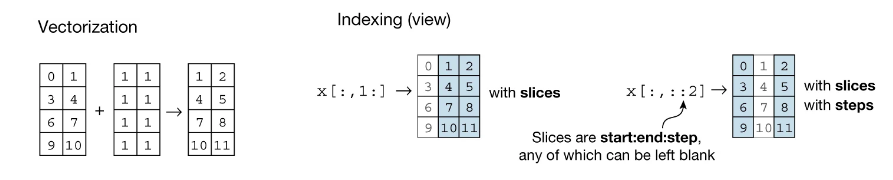
\includegraphics[width=\textwidth]{numpyoperations.png}
	\end{figure}


	More information can be found on the NumPy paper (Harris et al., Nature 2020) or on the NumPy website (www.numpy.org)
\end{frame}

\begin{frame}
	{Using Scikit Image to read and show images}

	In order to display an image saved in a NumPy array, we can use the Scikit Image library.

	\only<1-3>{
		\begin{codebox}
			\texttt
			{from skimage.io import imread, imshow\\
				\# Read the image\\
				img = imread("image.tif")\\
				\# Show the image\\
				imshow(img)\\
				\pause
				img\_small = img[0:5, 0:5]\\
				imshow(img\_small)\\
				\pause
				print(img.shape) \# Prints (10, 10)\\
				print(img\_small.shape) \# Prints (5, 5)
			}
		\end{codebox}
	}
	\only<4->{
		\begin{figure}
			\centering
			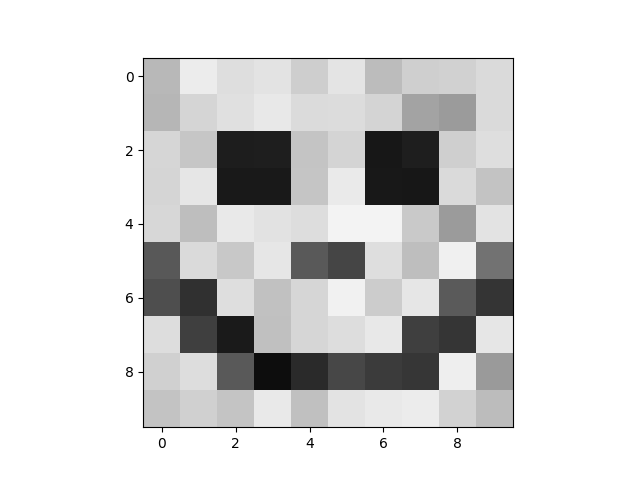
\includegraphics[height=140px]{smileyfull.png}
			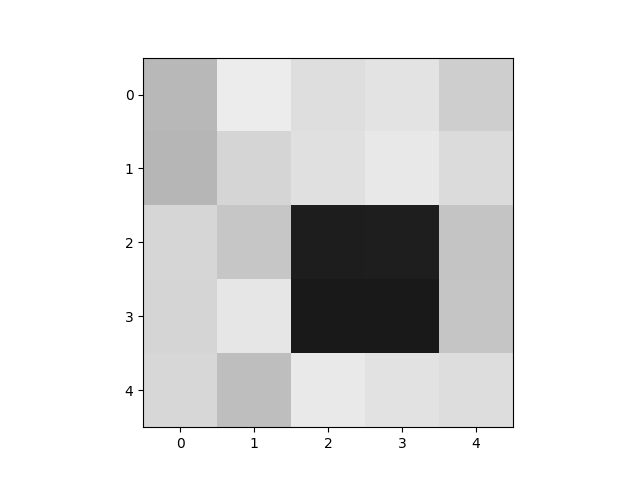
\includegraphics[height=140px]{smileytop.png}
		\end{figure}
	}
\end{frame}


\begin{frame}
	\Huge
	\centering
	Information in images
\end{frame}

\begin{frame}
	{Information in images - Resolution}
	Several parameters influence the amount of quantitative information present in an image.

	\begin{figure}
		\textbf{Resolution} is the number of pixels in the image.
		\centering
		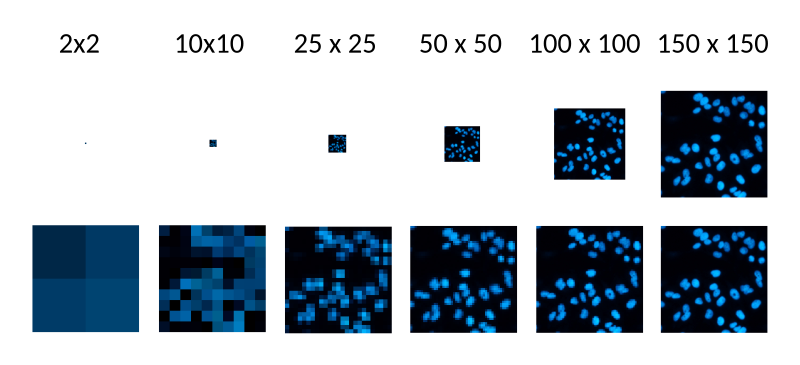
\includegraphics[width=\textwidth]{resolution.png}
		\caption{(Increasing resolution > Increasing information)}
	\end{figure}
\end{frame}

\begin{frame}
	{Information in images - Colour}
	Images can be either \textbf{colour} or \textbf{grayscale}.
	\begin{figure}
		\centering
		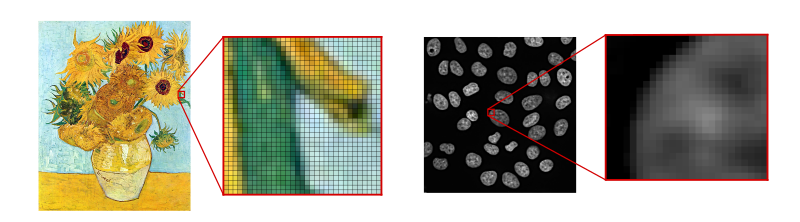
\includegraphics[width=\textwidth]{color_vs_grayscale.png}
		\caption{
			\centering
			\textbf{Colour} > each pixel contains information for red, green and blue (RGB)

			\textbf{Grayscale} > each pixel contains gray information (from black to white))}
	\end{figure}
	\centering
	\textbf{Most biomedical images are grayscale.}
\end{frame}

\begin{frame}
	{Information in images - Bit depth}
	\begin{figure}
		\textbf{Bit depth} is the number of bits necessary to represent each pixel in the image.
		\centering
		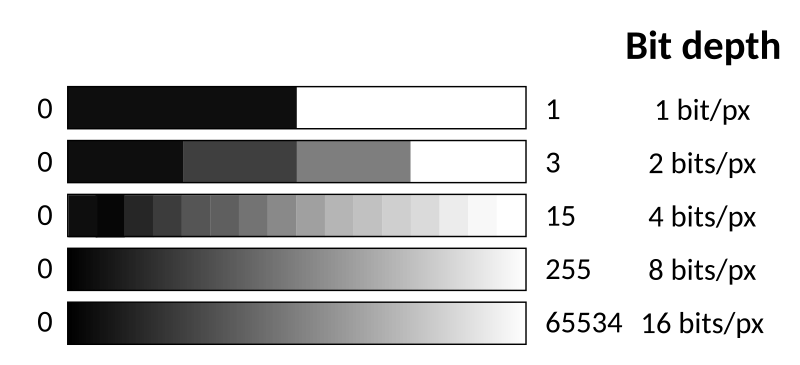
\includegraphics[width=.8\textwidth]{bitdepth.png}
		\caption{(Increasing bit depth > Increasing information)}
	\end{figure}

	Most often you will deal with 8- and 16-bits/pixel images (what most microscopes and cameras use) or 1 bit/pixel images, which are used as masks.
\end{frame}

\begin{frame}
	{Information in images - Formats and compression}
	There are a lot of file formats used for images.

	Images can be compressed or uncompressed. Compression can be lossless (e.g. LZW) or lossy (e.g. JPEG). Lossy compressed images should not be used as the base for quantitative imaging.
	\begin{figure}
		\centering
		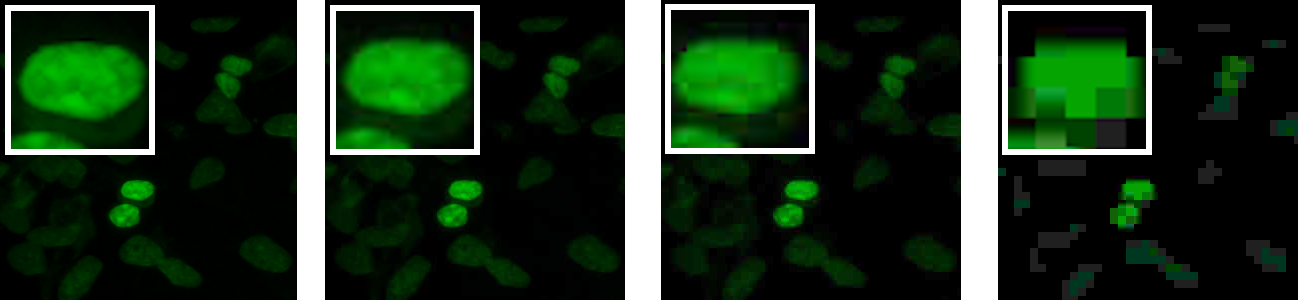
\includegraphics[width=380px]{compression.png}
		\caption{Increasing JPEG compression generates artefacts and loses information.}
	\end{figure}

	\pause
	\textbf{TIFF} is one of the most common image files used in biomedical sciences. Many microscopes save images in proprietary formats (e.g. Zeiss > CZI or Nikon > ND2). Newer formats such as \textbf{HDF5} and \textbf{Zarr} allow fast access to big data by allowing chunked access to data.
\end{frame}

\begin{frame}
	{Information in images - Metadata}
	Metadata is all non-image data contained in the file. For example when the image was taken, the instrument used, the wavelength and microscope filters used, a description of the experiment etc.

	\begin{figure}
		\centering
		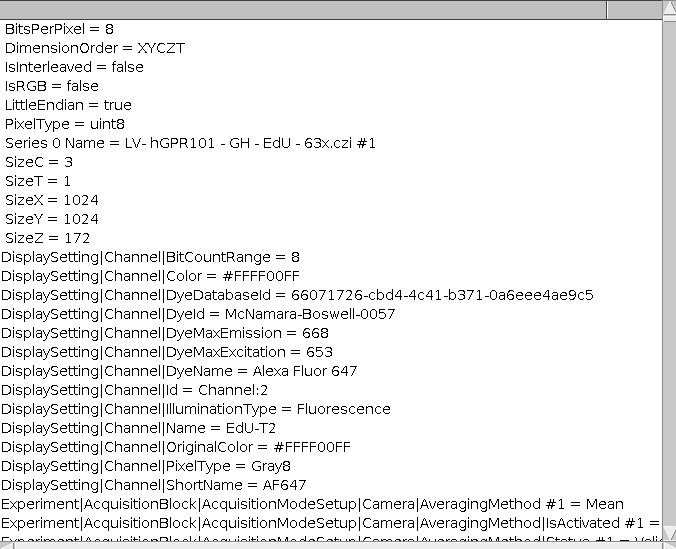
\includegraphics[height=180px]{metadata.png}
	\end{figure}
\end{frame}

\begin{frame}
	\Huge
	\centering
	Colouring
\end{frame}

\begin{frame}
	{Pseudocoloring}
	Often colour is applied to microscopic images \textbf{after} acquisition to mark different parts of the image. This is called \textbf{pseudocolouring} or \textbf{false colouring}.
	\begin{figure}
		\centering
		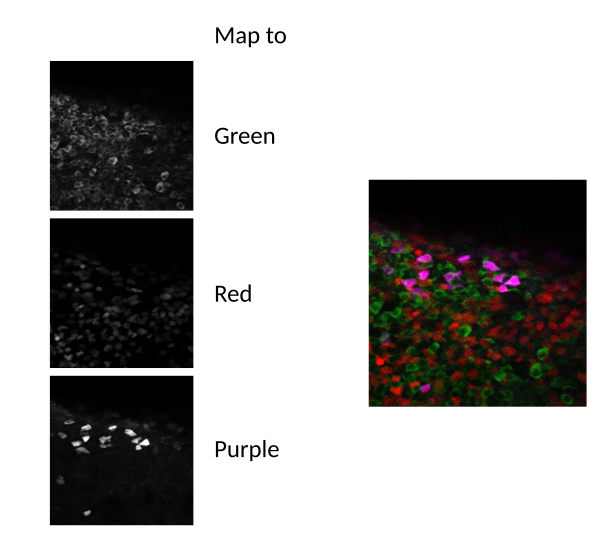
\includegraphics[height=180px]{pseudocolor.png}
	\end{figure}
\end{frame}

\begin{frame}
	{Look-up tables (LUTs)}
	Pseudocoloring is obtained through look-up tables (sometimes referred to as "palettes" or "colourmaps")

	\begin{figure}
		\centering
		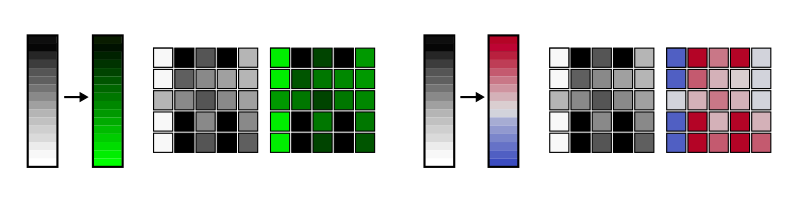
\includegraphics[width=400px]{lut.png}
		\caption{\centering Colourmaps can be sequential/linear or non sequential.

			Divergent and non linear colour maps can be good to enhance differences in the image,

			but should be used with caution!}
	\end{figure}
\end{frame}

\begin{frame}
	{The Jet palette - when colourmaps go bad...}
	The Jet colourmap has for a long time been the standard palette in Matlab, is used in many pieces of software and is seen in many published articles. Jet is problematic because it can create artefacts in your data.

	\begin{figure}
		\centering
		\only<1>
		{
			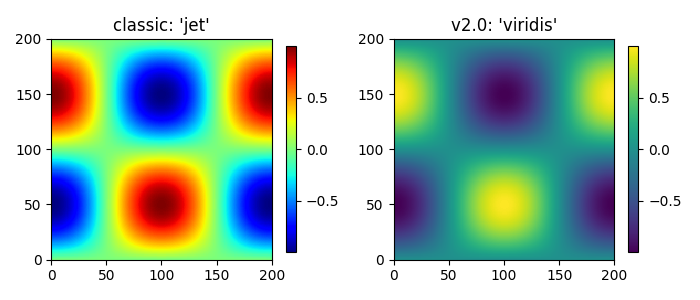
\includegraphics[width=300px]{jet_vs_viridis.png}
			\caption{\centering
				Jet can create artefacts in the data. [Source: Matplotlib website]

				See https://www.youtube.com/watch?v=xAoljeRJ3lU}
		}
		\only<2>
		{
			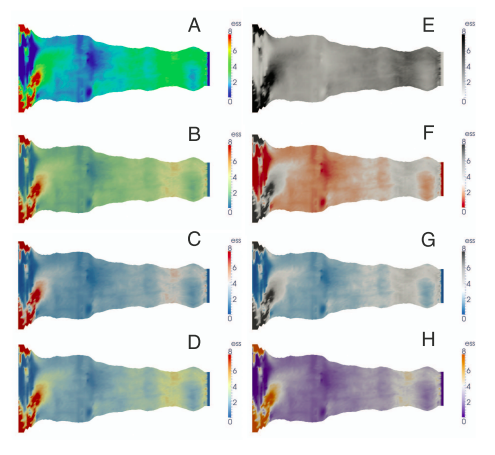
\includegraphics[width=170px]{borkin2011.png}
			\caption{\centering
				\textit{Rainbow} palette resulted in significantly more diagnostic errors - Borkin 2011}
		}
	\end{figure}
\end{frame}

\begin{frame}
	{Colourmapping in Matplotlib}
	We can easily colourmap an image loaded in Matplotlib

	\only<1-2>{
		\begin{codebox}
			\texttt{\# We will use the Matplotlib library this time\\
				import matplotlib.pyplot as plt\\
				from skimage.io import imread\\
				\\
				img = imread("smiley.tif")\\
				\# plt.subplots allows plotting more than one image\\
				\# side by side. It creates and returns a figure and\\
				\# a list of axes (the subplots)\\
				fig, ax = plt.subplots(ncols=3, nrows=1, figsize=(10, 5))\\
				\pause
				ax[0].imshow(img, cmap="viridis")\\
				ax[1].imshow(img, cmap="terrain")\\
				ax[2].imshow(img, cmap="spring")\\
				plt.show()}
		\end{codebox}
	}
	\only<3>{
		\begin{figure}
			\centering
			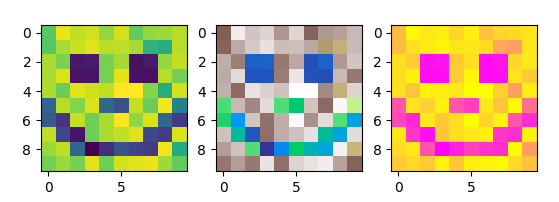
\includegraphics[width=\textwidth]{colourmaps.png}
		\end{figure}
	}
\end{frame}

\begin{frame}
	{Image histograms}
	An easy way to describe an image is to use a histogram. For each intensity level, we count the number of pixels that have that intensity.

	\begin{figure}
		\centering
		\only<1>
		{
			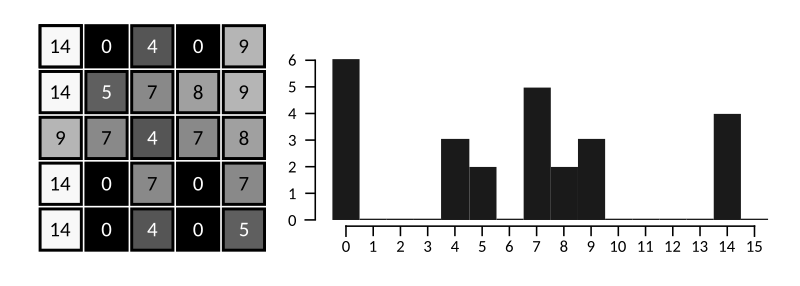
\includegraphics[height=150px]{simple_histogram.png}
		}
		\only<2>
		{
			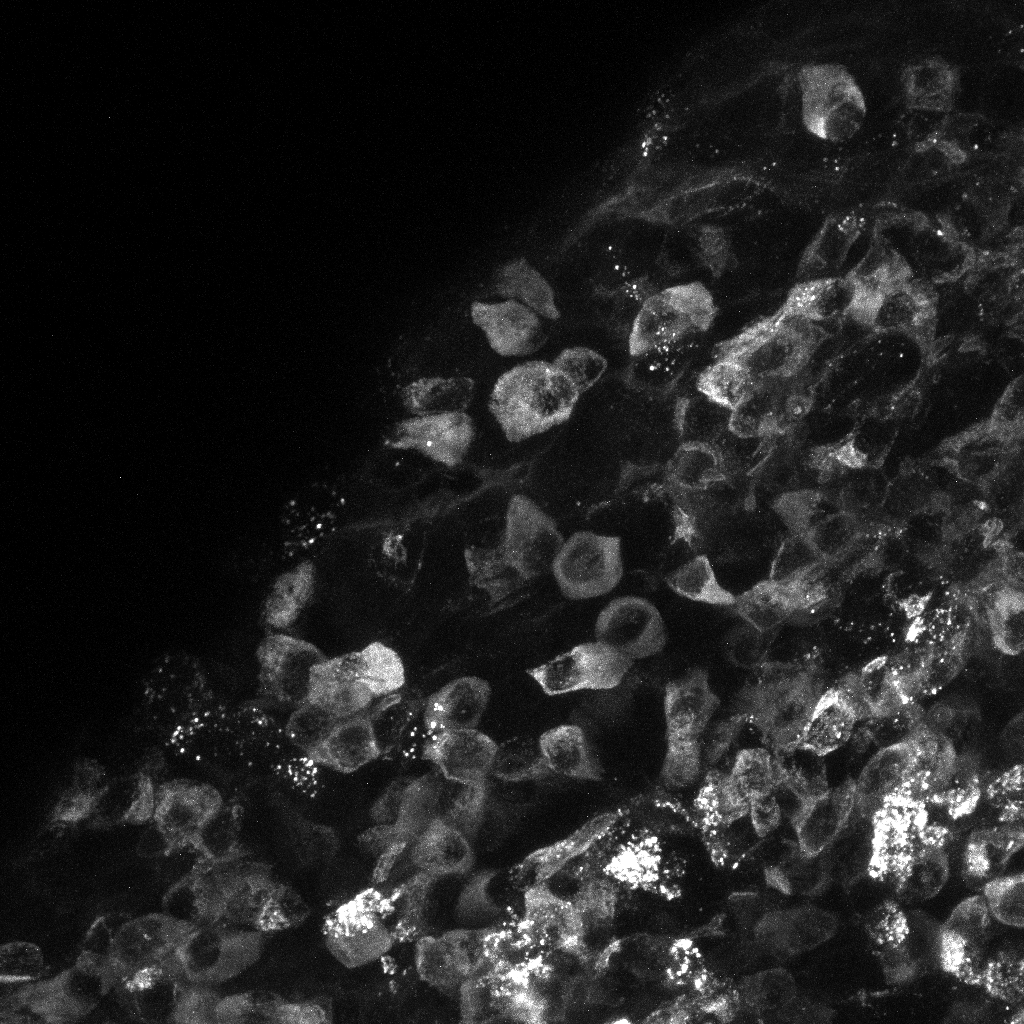
\includegraphics[height=150px]{cellshisto.png}
			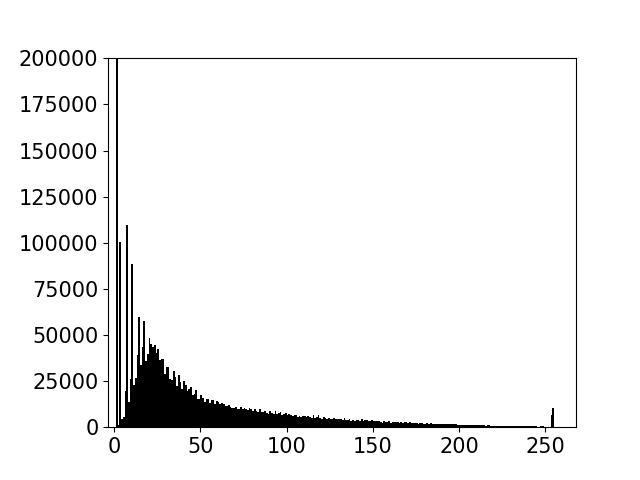
\includegraphics[height=160px]{histo.png}
		}
	\end{figure}
\end{frame}

\begin{frame}
	{Plotting a histogram using Matplotlib}

	\begin{codebox}
		\texttt{nuclei = imread("nuclei.tif")\\
			imshow(nuclei, cmap="gray")\\
			plt.hist(nuclei.ravel(), bins=range(255))\\
			plt.show()}
	\end{codebox}

	\begin{figure}
		\centering
		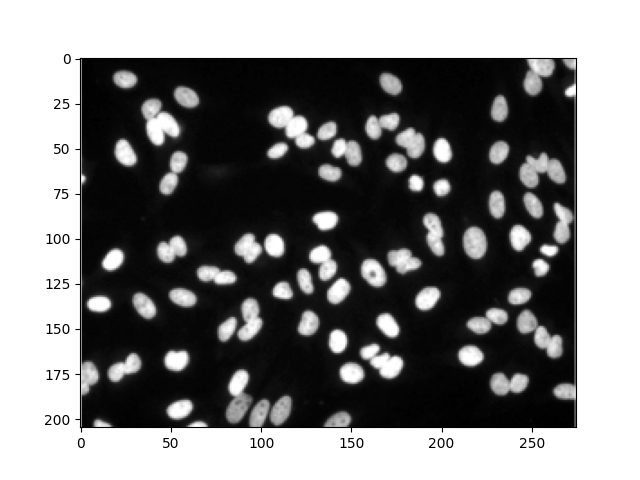
\includegraphics[width=.4\textwidth]{nuclei.png}
		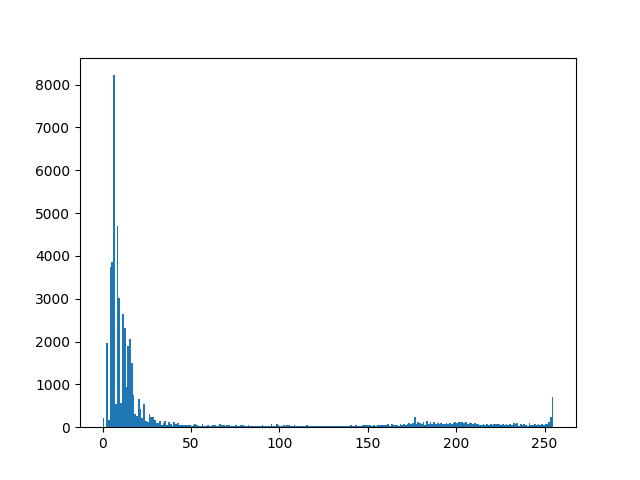
\includegraphics[width=.4\textwidth]{histonuclei.png}
	\end{figure}
\end{frame}

\begin{frame}
	{Over- and under-exposure}
	Histograms are a great tool to check the quality of your image. When adjusting the acquisition parameters on a microscope, care should be taken to use as much of the dynamic range as possible to avoid losing information. Although there are techniques to improve this after the fact... remember that \textit{garbage in, garbage out!}
	\begin{figure}
		\centering
		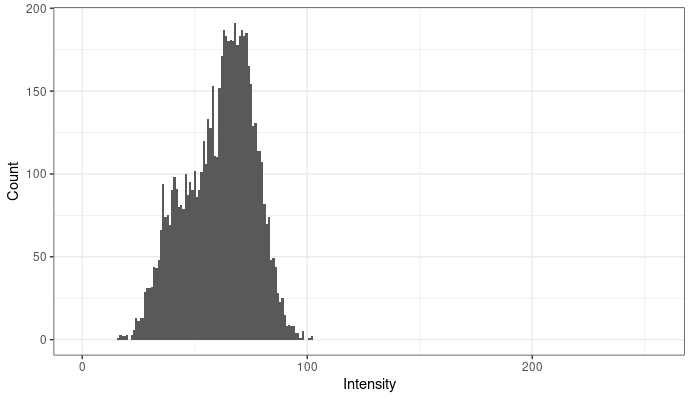
\includegraphics[width=130px]{underexposed.png}
		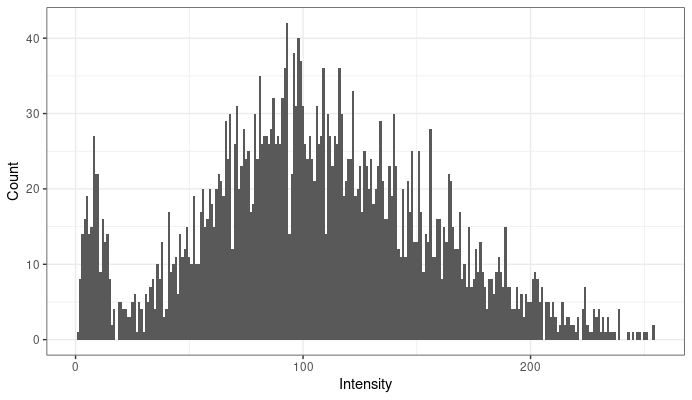
\includegraphics[width=130px]{normalexp.png}
		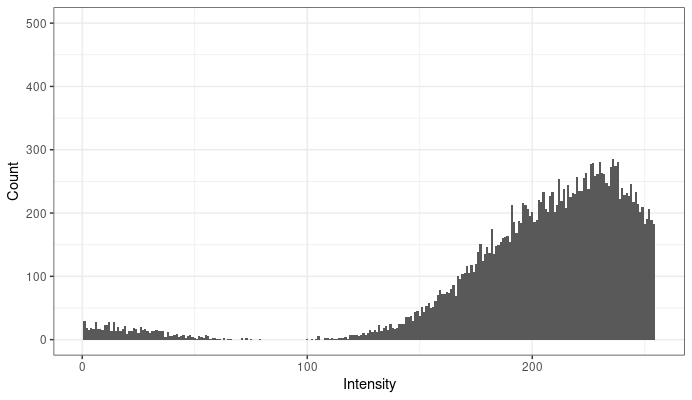
\includegraphics[width=130px]{overexposed.png}
	\end{figure}
\end{frame}

\begin{frame}
	{Brightness and contrast}
	\begin{itemize}
		\item \textbf{Brightness} is the overall lightness or darkness of an image.
		\item \textbf{Contrast} is the difference in brightness between different objects or regions of the image. Often we consider the difference in brightness between the experimental sample and the background.
	\end{itemize}
	\only<2>
	{
		\begin{figure}
			\centering
			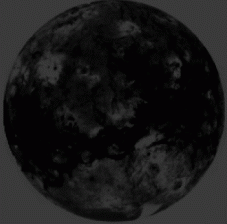
\includegraphics[width=100px]{lowbright.png}
			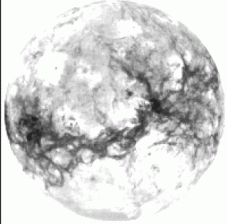
\includegraphics[width=100px]{highbright.png}
			\caption{
				\centering
				Low and high brightness versions of the same image. The left image is underexposed, while the right image is overexposed. [Source: Digital Signal Processing - S. W. Smith]
			}
		\end{figure}
	}
	\only<3>
	{
		\begin{figure}
			\centering
			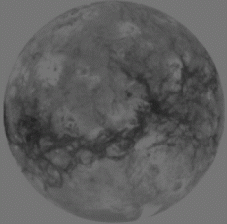
\includegraphics[width=100px]{lowcont.png}
			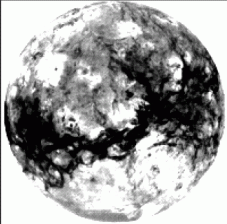
\includegraphics[width=100px]{highcont.png}
			\caption{
				\centering
				Low and high contrast versions of the same image. The left image has low contrast, so it is more difficult to distinguish the object from the background. [Source: Digital Signal Processing - S. W. Smith]
			}
		\end{figure}
	}
\end{frame}

\begin{frame}
	{Noise}
	Noise is an aspect that \textbf{decreases} the amount of information contained in an image. There are several sources of noise:
	\begin{itemize}
		\item Low amount of light
		      \begin{itemize}
			      \item In microscopy because of low intensity staining or because of low power light or other microscope settings.
			      \item In images taken with a camera because of low-ambient light.
		      \end{itemize}
		      \pause
		\item Shot noise. This is due to fluctuations of the number of photons detected by the system due to the dual wave/particle nature of light.
		\item Detector noise. In digital images, this is due to the inherent noise of the sensor, because of electronic circuit noise, temperature, etc
		      \pause
		\item Autofluorescence of sample. Particularly problematic for green and red wavelengths; non-biological debris often fluoresce strongly in the UV. Far-red and infrared less affected.
		\item Ambient light interference.
	\end{itemize}
\end{frame}
\begin{frame}
	{Noise and loss of information}
	Noise can mask important information in a signal. \textbf{Signal-to-noise ratio (SNR)} is a measure of the intensity of the signal we are trying to measure compared to the noise.
	\begin{figure}
		\centering
		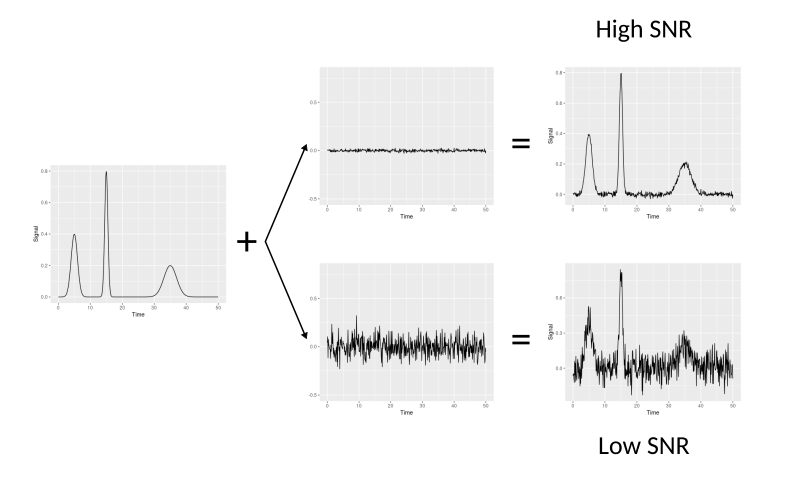
\includegraphics[width=.8\textwidth]{signal_noise.png}
	\end{figure}
\end{frame}

\begin{frame}
	{SNR in images}
	There are different, domain-specific ways of calculating SNR; for biomedical images it is often useful to consider the area containing the sample as signal and the background as "noise".

	\large
	$SNR = 10*log_{10}\frac{\mu_{signal}}{\sigma_{noise}}$
	\begin{figure}
		\centering
		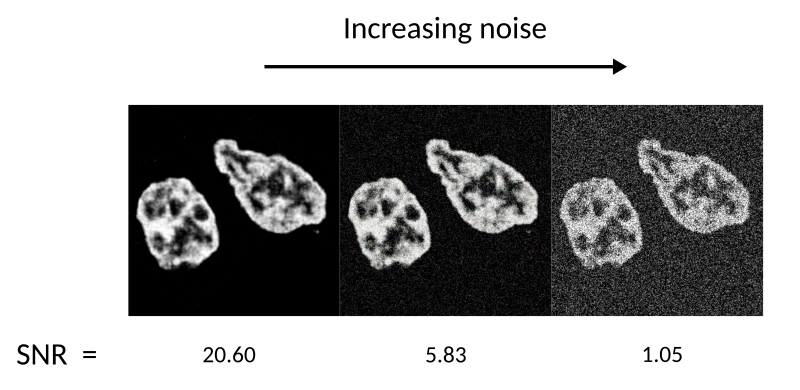
\includegraphics[width=.8\textwidth]{noisyimage.png}
	\end{figure}
\end{frame}

\begin{frame}
	{Summary}
	Images are used as an important source of information in biomedical sciences.

	Quantitative imaging relies on the representation of images as n-dimensional matrices of pixels.

	Python provides tools for dealing with matrices (e.g. numpy) and for image analysis in general.

	Information depends on many aspects of the image and

	Next lecture will deal with some basic, but important preprocessing steps that you will use in most image analysis workflows.
\end{frame}
\end{document}